\section{Datasets, MC samples and event selection}
\label{sec:Datasets}

\subsection{Datasets}
This analysis is performed using the \textbf{Ultra Legacy} 2017 $\pp$ data at $\sqrtsNN$=5.02 TeV, which has an integrated luminosity of 302.3 $pb^{-1}$.  %The pp reference is using the 2015 pp  at $\sqrtsNN$=5.02 TeV data. The details of the 2015 $B_{S}$ pp data analysis can be found in ~\cite{AN-17-210}.   
%The proton-proton dataset corresponds to an integrated luminosity of 28.0 pb$^{-1}$
The analysis uses the dimuon primary datasets (\textit{DoubleMu} PD). The full name of the used datasets can be found in Table~\ref{tab:lumi}.

\begin{table}[htb]
\begin{center}
\caption{List of pp HLT datasets and triggers with the corresponding integrated luminosities used in the analysis.}
\label{tab:lumi}
 \tiny
 \begin{tabular}{ l | l | l | l | }
 System& Primary dataset & Trigger & Luminosity\\
  \hline\hline
% $\pp$ & \verb#HiOniaDoubleMu0/HIRun2015-PromptReco-v1/AOD# & \verb#HLT_HIL1DoubleMu0_v1# & $135.64\mubinv$ \\
 % $\pp$ & \verb#HiOniaDoubleMu0B/HIRun2015-PromptReco-v1/AOD# & \verb#HLT_HIL1DoubleMu0_part1_v1# & $71.71\mubinv$ \\
 % $\pp$ & \verb#HiOniaDoubleMu0C/HIRun2015-PromptReco-v1/AOD# & \verb#HLT_HIL1DoubleMu0_part2_v1# & $71.67\mubinv$ \\
 % $\pp$ & \verb#HiOniaDoubleMu0D/HIRun2015-PromptReco-v1/AOD# & \verb#HLT_HIL1DoubleMu0_part3_v1# & $71.67\mubinv$ \\
 
	 $\pp$ & \verb#/DoubleMuon/Run2017G-09Aug2019_UL2017-v1/AOD# & \verb# HLT_HIL3Mu0NHitQ10_L2Mu0_MAXdR3p5_M1to5_v1 # & $302.3 pb^{-1}$\\

  \hline

  %\hline\hline
  %$\pp$ & \verb#/DoubleMu/Run2015E-PromptReco-v1/AOD# & \verb#HLT_HIL1DoubleMu0_v1# & $27.70\pbinv$ \\
 \end{tabular}
\end{center}
\end{table}

%The pp analysis codes are running under the CMSSW\_7\_5\_8\_patch3 version, and the global tag (GT) used for processing these samples is auto:run\_2 data. \\ \\
The pp analysis codes are running under the CMSSW\_9\_4\_10\ version, and the global tag (GT) used for processing these samples is 94X\_dataRun2\_ReReco\_EOY17\_v6. \\ \\
Events used in the measurement are collected with a trigger requiring the presence of two independent muon candidates.
No selection is applied on momentum (including transverse momentum) or pseudo-rapidity.
A list of the various triggers with the corresponding integrated luminosities can be found in Table~\tab{tab:lumi}.
%The pp HLT trigger path was unprescaled during the whole run
The $\pp$ paths had different prescale values in different runs during the data taking period. 
A complete description of the di-muon datasets and HLT triggers can be found in~\cite{AN-16-067}.

Muon JSON file is applied to filter the pp dataset. It can be found at: Cert_306546-306826_5TeV_EOY2017ReReco_Collisions17_JSON_MuonPhys.txt.

\subsection{Event Selection}
\label{sec:data.filter}
To extract pure collision events, several offline selections are applied to each event:
\begin{itemize}
\item \verb|pPAprimaryVertexFilterNew|: Events are required to have at least one reconstructed primary vertex.
  The primary vertex is formed by two or more associated tracks and is required to have a distance from the
  nominal interaction region of less than 15\cm along the beam axis and less than 0.15\cm in the transverse plane.
\item \verb|HBHENoiseFilterResult|: An additional selection of hadronic collisions is applied by requiring a coincidence of at least 2 HF calorimeter towers,
  with more than 4\gev of total energy, from the HF detectors on both sides of the interaction point.
\item \verb|pBeamScrapingFilterNew|: In addition to HF coincidence, a cluster compatibility filter is used
\item \verb|HLT_HIL1DoubleMu0_v1New|: dimuon triggered events

\end{itemize}
%There is also a requirement on the centrality (hiBin) of the events to selection only 0 - 90\% centrality class events: hiBin$<$181.

In addition, we also require the absolute value of the z-component of the primary vertex position to be $\abs{PV_z} <$ 15 cm.
\subsection{MC samples}
\label{sec:mcsample}
%The $\pp$ sample is reconstructed using the CMSSW version CMSSW\_7\_5\_8\_patch3.
The $\pp$ sample is reconstructed using the CMSSW version CMSSW\_9\_4\_10 using the \textbf{Ultra Legacy} reconstruction procedures.
The global tag used for the production is \verb!94X_mc2017_realistic_forppRef5TeV! for pp samples.
Dedicated pp \PBzs samples were generated in order to estimate the acceptance and selection efficiencies, to study the background components, and to evaluate systematic uncertainties. 
{\sc PYTHIA8} Tune CUETPM8~\cite{pythia,Field:2010bc}, set to generate inclusive (all quark/antiquark, as well as gluon initiated) QCD processes, was used to generate at 5.02 TeV the signal. Several prefilters at the generation steps are applied in order to optimize the generation process and conserve resources.
Only signal events were kept with at least one \PBzs (forced to decay through the channel \bspsiphi by means of the {\sc evtgen} package~\cite{Lange:2001uf}), with $\pt>$5.0$\GeVc$, and $|\eta|<$2.4.
In addition, the $\Jpsi$ and $\phi$ meson, are forced to decay in the two muons and two kaons respectively.
Final state radiations (FSR) are generated using {\sc photos}~\cite{Barberio:1990ms}.
The selected signal is simultated with PYTHIA 8 pp cillisions  %(version 1.8, tune "Drum" for the prompt and non-prompt \JPsi MC and tune "Cymbal5Ev8" for the \PBzs signal MC)~\cite{Lokhtin:2005px} event generator.

Around 2.5 million events were generated in 1 $\hat{p}_{T} > 5$ bin. The list of \PBzs and \PB MC simulation samples used are shown below:


\begin{itemize}
	\tiny \item $B^{0}_s$: \verb#/BsToJpsiPhi_pThat-5_TuneCP5_5p02TeV_Pythia8/RunIIpp5Spring18DR-94X_mc2017_realistic_forppRef5TeV_v1-v4/AODSIM#\\
	      \item $B^{+}$:    \verb#/BsToJpsiPhi_pThat-5_TuneCP5_5p02TeV_Pythia8/RunIIpp5Spring18DR-94X_mc2017_realistic_forppRef5TeV_v1-v4/AODSIM#\\
\end{itemize}

In addition to the signal samples, inclusive non-prompt \JPsi samples, which include several different \PB\ meson decaying to \JPsi channels, were also generated.
These samples were used to determine the peaking background appearing in the \Pgm\Pgm\PK\PK\  mass spectrum. The following samples were used:

\begin{itemize}
\tiny \item \verb#/Pythia8_BJpsiMM_ptJpsi_00_03_Hydjet_MB/HINppWinter16DR-75X_mcRun2_HeavyIon_v13-v1/AODSIM# 
\item  \verb#/Pythia8_BJpsiMM_ptJpsi_03_06_Hydjet_MB/HINppWinter16DR-75X_mcRun2_HeavyIon_v13-v1/AODSIM# 
\item  \verb#/Pythia8_BJpsiMM_ptJpsi_03_06_Hydjet_MB/HINppWinter16DR-75X_mcRun2_HeavyIon_v13_ext1-v1/AODSIM# 
\item  \verb#/Pythia8_BJpsiMM_ptJpsi_06_09_Hydjet_MB/HINppWinter16DR-75X_mcRun2_HeavyIon_v13-v1/AODSIM# 
\item  \verb#/Pythia8_BJpsiMM_ptJpsi_06_09_Hydjet_MB/HINppWinter16DR-75X_mcRun2_HeavyIon_v13_ext1-v1/AODSIM# 
\item  \verb#/Pythia8_BJpsiMM_ptJpsi_09_12_Hydjet_MB/HINppWinter16DR-75X_mcRun2_HeavyIon_v13-v1/AODSIM# 
\item  \verb#/Pythia8_BJpsiMM_ptJpsi_12_15_Hydjet_MB/HINppWinter16DR-75X_mcRun2_HeavyIon_v13-v1/AODSIM# 
\item  \verb#/Pythia8_BJpsiMM_ptJpsi_15_30_Hydjet_MB/HINppWinter16DR-75X_mcRun2_HeavyIon_v13-v1/AODSIM# 
\item  \verb#/Pythia8_BJpsiMM_ptJpsi_30_inf_Hydjet_MB/HINppWinter16DR-75X_mcRun2_HeavyIon_v13-v1/AODSIM# 

\end{itemize}

The inclusive non-prompt  \JPsi samples are also used in the $B^+$ analysis to constrain the non-prompt background.

Finally, the following prompt \JPsi samples were used:

\begin{itemize}
\tiny \item  \verb#/Pythia8_JpsiMM_ptJpsi_00_03_Hydjet_MB/HINppWinter16DR-75X_mcRun2_HeavyIon_v13-v1/AODSIM# 
\item  \verb#/Pythia8_JpsiMM_ptJpsi_03_06_Hydjet_MB/HINppWinter16DR-75X_mcRun2_HeavyIon_v13-v1/AODSIM# 
\item  \verb#/Pythia8_JpsiMM_ptJpsi_03_06_Hydjet_MB/HINppWinter16DR-75X_mcRun2_HeavyIon_v13_ext1-v1/AODSIM# 
\item  \verb#/Pythia8_JpsiMM_ptJpsi_06_09_Hydjet_MB/HINppWinter16DR-75X_mcRun2_HeavyIon_v13-v1/AODSIM# 
\item  \verb#/Pythia8_JpsiMM_ptJpsi_06_09_Hydjet_MB/HINppWinter16DR-75X_mcRun2_HeavyIon_v13_ext1-v1/AODSIM# 
\item  \verb#/Pythia8_JpsiMM_ptJpsi_09_12_Hydjet_MB/HINppWinter16DR-75X_mcRun2_HeavyIon_v13-v1/AODSIM# 
\item  \verb#/Pythia8_JpsiMM_ptJpsi_12_15_Hydjet_MB/HINppWinter16DR-75X_mcRun2_HeavyIon_v13-v1/AODSIM# 
\item  \verb#/Pythia8_JpsiMM_ptJpsi_15_30_Hydjet_MB/HINppWinter16DR-75X_mcRun2_HeavyIon_v13-v1/AODSIM# 
\item  \verb#/Pythia8_JpsiMM_ptJpsi_30_Inf_Hydjet_MB/HINppWinter16DR-75X_mcRun2_HeavyIon_v13-v1/AODSIM# 
\end{itemize}

\clearpage

\subsubsection{MC reweighting}
\label{sec:mcreweighting}

\iffalse 
The ratio between the MC and the various different spectra shape as shown in the right panel of the same figure. 

\begin{figure}[h]
\begin{center}
\includegraphics[width= 0.95\textwidth]{Plots/Results/plotReweight/canvasPtReweightpp_NominalPP.pdf}
\includegraphics[width= 0.95\textwidth]{Plots/Results/plotReweight/canvasPtReweightpp_VariationPP.pdf}
\includegraphics[width= 0.95\textwidth]{Plots/Results/plotReweight/canvasPtReweightpp_NominalTAMU.pdf}
\includegraphics[width= 0.95\textwidth]{Plots/Results/plotReweight/canvasPtReweightpp_VariationTAMU.pdf}
\caption{ \PBzs \pt spectrum obtained in pp MC simulations (left panel) compared to the one obtained in Nominal PP (best $\chi^2$), Variation PP (second best $\chi^2$), Nominal TAMU (Nominal PP $\times$ TAMU $R_{AA}$), and Variation TAMU (Variation PP $\times$ TAMU $R_{AA}$)  calculations at 5.02 TeV (from up to down). 
Ratio between the MC and FONLL and NLO distributions, fitted with the sum between an exponential function and constant offset function (right).}
\label{fig:datamc-genpt-pp}
\end{center}
\end{figure}
\fi





For our MC reweighting, we reweight our MC directly to our data shape in the RECO level. We extract the data raw yield from the unbinned fit and the MC raw yield by count the total number of MC candidates with $\hat \pt$, $PV_z$, and centrality reweighting. The $J\psi$, $B^+$, and $B_s$ Gen \pt distribution before and after are shown below on Fig ~\ref{fig:pthatWeightPlot} 

\begin{figure}[h]
\begin{center}

\includegraphics[width= 0.30\textwidth]{Plots/MCReweight/GenInfo/BPpthat.png}

\includegraphics[width= 0.30\textwidth]{Plots/MCReweight/GenInfo/BPJPsiPt.png}
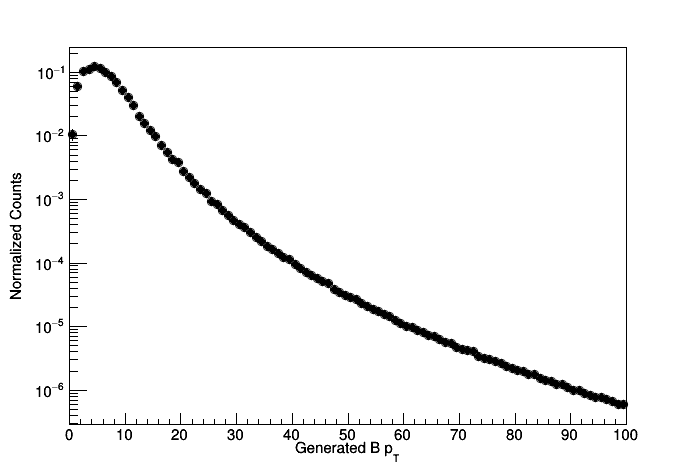
\includegraphics[width= 0.30\textwidth]{Plots/MCReweight/GenInfo/BPGpt.png}

\includegraphics[width= 0.30\textwidth]{Plots/MCReweight/GenInfo/Bspthat.png}

\includegraphics[width= 0.30\textwidth]{Plots/MCReweight/GenInfo/BsJPsiPt.png}
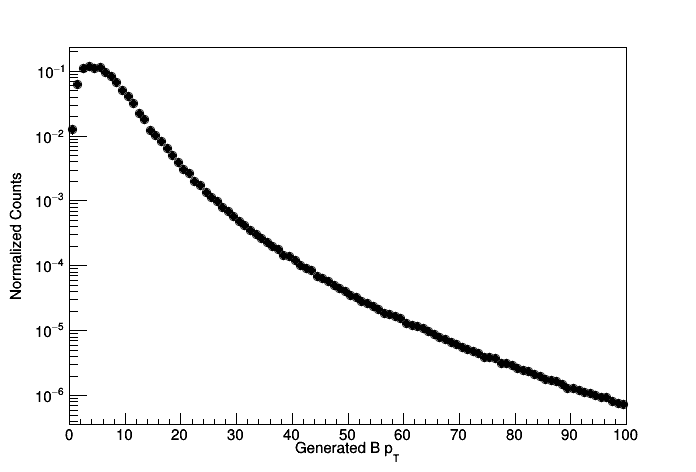
\includegraphics[width= 0.30\textwidth]{Plots/MCReweight/GenInfo/BsGpt.png}
\caption{The pthat distribution of the official MC sample (left) as well as the generated $J/\psi$ (middle) and B-meson \pt distribution with pthat weight applied of $B^{+}$ and $B^0_s$ are shown respectfully above.}
\label{fig:pthatWeightPlot}
\end{center}
\end{figure}

We can see that after $\hat \pt$ reweighting, the Gen \pt distributions have become smoother. This validate our $\hat \pt$ reweighting procedures. 


%Then, we take the ratio of the normalized data raw yield to the normalized MC raw yield and perform a variety of functions to fit the distribution. In our studies, we use Linear ($y = p_0 + p_1 x$), Quadratic ($y = p_0 + p_1 x + p_2 x^2$), Linear + Inverse  ($y = p_1 x + \frac{p_2}{x}$), Linear + Square Root ($y = p_0 + p_1 x + p_2 \sqrt{x}$), Linear + Log ($y = p_0 + p_1 x + p_2 \log{x}$). The data vs MC raw yield shape and our fitting results on spectra ratio are show as follows on Fig~ \ref{fig:BptReweightShape}

Then, we take the ratio of the normalized data raw yield to the normalized MC raw yield and perform a fit with function: $y = p_0/x^2 + p_1 log(x) + p_2$. Our fitting results on spectra ratio are show as follows on Fig~ \ref{fig:BptReweightShape}


\begin{figure}[h]
\begin{center}
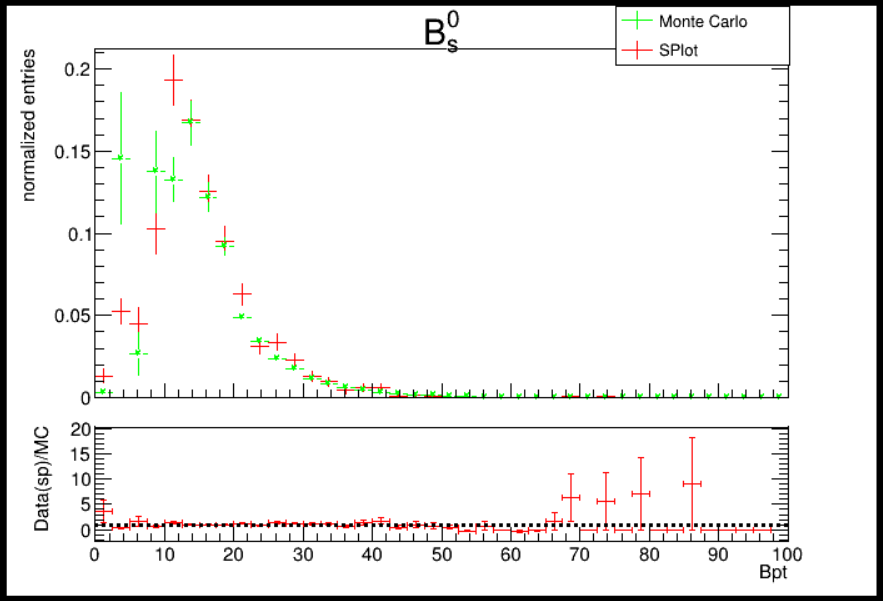
\includegraphics[width= 0.45\textwidth]{Plots/MCReweight/Bpt/BPPtDataMC.png}
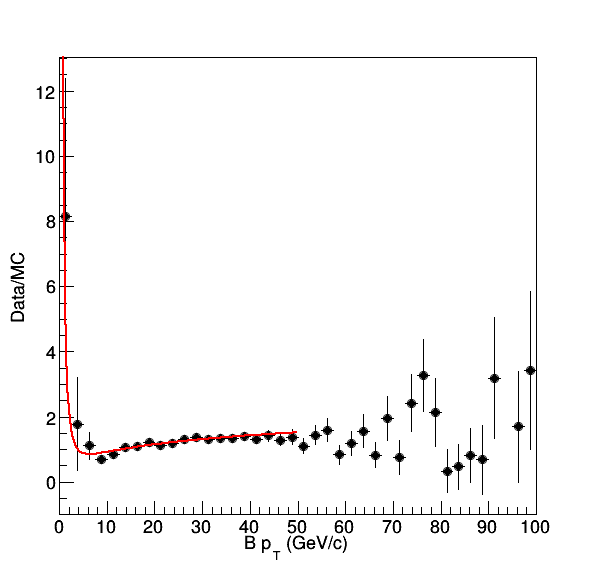
\includegraphics[width= 0.45\textwidth]{Plots/MCReweight/Bpt/BPPtWeight.png}
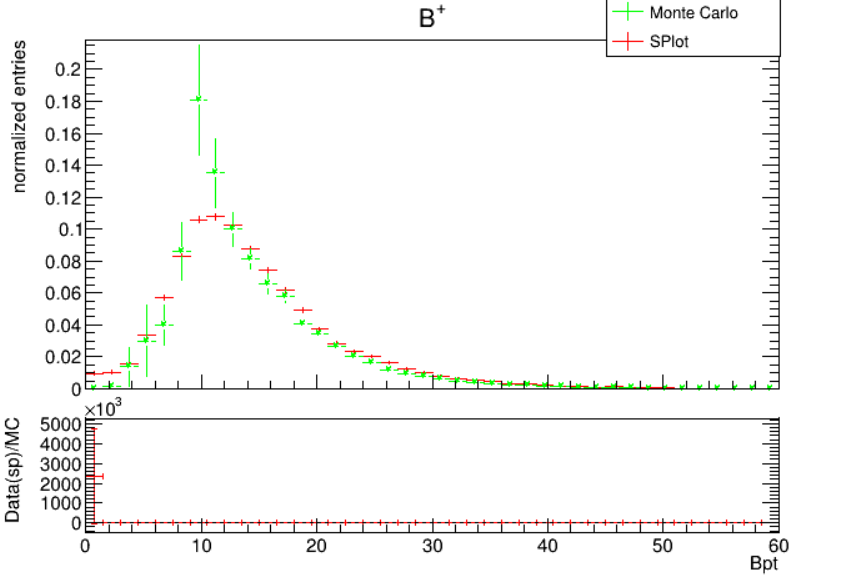
\includegraphics[width= 0.45\textwidth]{Plots/MCReweight/Bpt/BsPtDataMC.png}
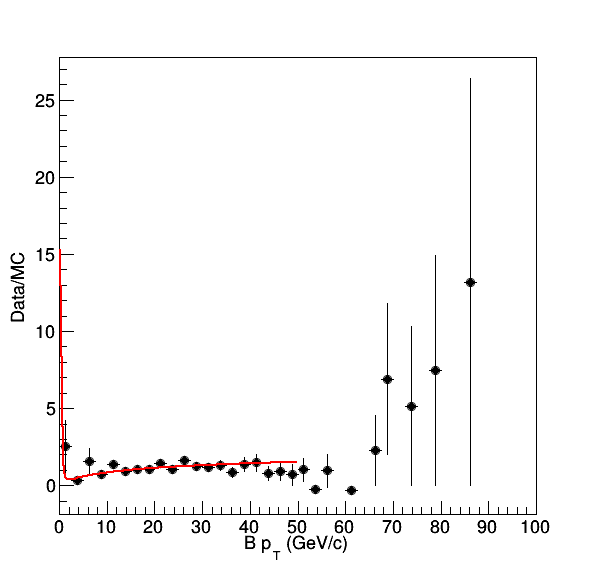
\includegraphics[width= 0.45\textwidth]{Plots/MCReweight/Bpt/BsPtWeight.png}
\caption{The MC-Data agreement between the signal raw yield in data (red) and MC (green) as a function of B meson $p_{T}$ for $B^{+}$ (up) and $B^0_s$ (down). We fit the ratio with the function: $y = p_0/x^2 + p_1 log(x) + p_2$. We will apply this function to the efficiency correct to obtain the systematic uncertainties due to the B $p_T$ shapes.}
\label{fig:BptReweightShape}
\end{center}
\end{figure}


The fitting parameters for all functions are shown below on Table~ \ref{fig:BptReweighTable}



\begin{table}[h]
\begin{center}
\caption{Summary of fitting parameters for the fitting functions of $B^+$ and $B^0_s$ above is shown below.}
\vspace{1em}
\label{fig:BptReweighTable}
\begin{tabular}{| c | c | c | c| }
\hline
Particles & $p_0$ & $p_1$ & $p_2$  \\
\hline
$B^{+}$ &  8.65  &  4.26 & -1.48  \\
$B^0_s$  &  1.00 & 0.436 & 0.171    \\
\hline
\end{tabular}
\end{center}
\end{table}

\clearpage




In addition to above pt shape and centrality reweighting, there must be a primary vertex z position (PVz) reweighting.
It is known there will be some non-trivial disagreement on the primary vertex between data and MC simulated with PYTHIA 8. Also, the offsets between data and MC in the X and Y directions are observed in the 2017 pp collisions. A Gaussian fit is applied to both the data and MC PVz distributions, as showed in Fig.~\ref{fig:datamc-pvz-pp}. The blue markers represent the distribution points for data (left) and MC (middle), while the red lines represents the Gaussian fit results. \note{Add table with fit results} Then, the ratio between the two fit results is taken as the weighting function. Finally, we use the ratio function of reweigh the MC and plot the reweighted MC along with the data on the right window. 
The result after this weighting can be found in Fig. \ref{fig:datamc-pvz-pp} for $B^+$ (up) and $B^0_s$ (down). The Gaussian fit results are given by:

\begin{table}[h]
\begin{center}
	\caption{Summary of fitting parameters for the Gaussian functions ($y = N e^{\frac{-(x-\mu)^2}{2 \sigma^2}}$) of $B^+$ and $B^0_s$ }
\vspace{1em}
\label{fig:BptReweighTable}
\begin{tabular}{| c | c | c | c| }
\hline
	Gaussian Fitting Parameters & N & $\mu$ & $\sigma$ \\
\hline
$B^+$ Data & 0.0132  &  0.7538 & 6.024 \\
$B^+$ MC &  0.0137 & 0.6197 & 5.813 \\
$B^0_s$ Data &  0.0132 & 0.7539 & 6.024  \\
$B^0_s$ MC &  0.0137 & 0.6205 & 5.815    \\
\hline
\end{tabular}
\end{center}
\end{table}



%On the right is the ratio between MC and data, a good agreement is observed.

But note that this analysis is not sensitive to the absolute value of the PV position because the reconstruction of the \Bs meson rely only on the relative distance between PV and \Bs reconstructed vertex which is presented in the following section.
%\textcolor{red}{We tried to estimate this effect by removing this re-weighting entirely and found that the difference is only 1.3\%.}\comment{Do we need to calculate this?}

\begin{figure}[h]
\begin{center}
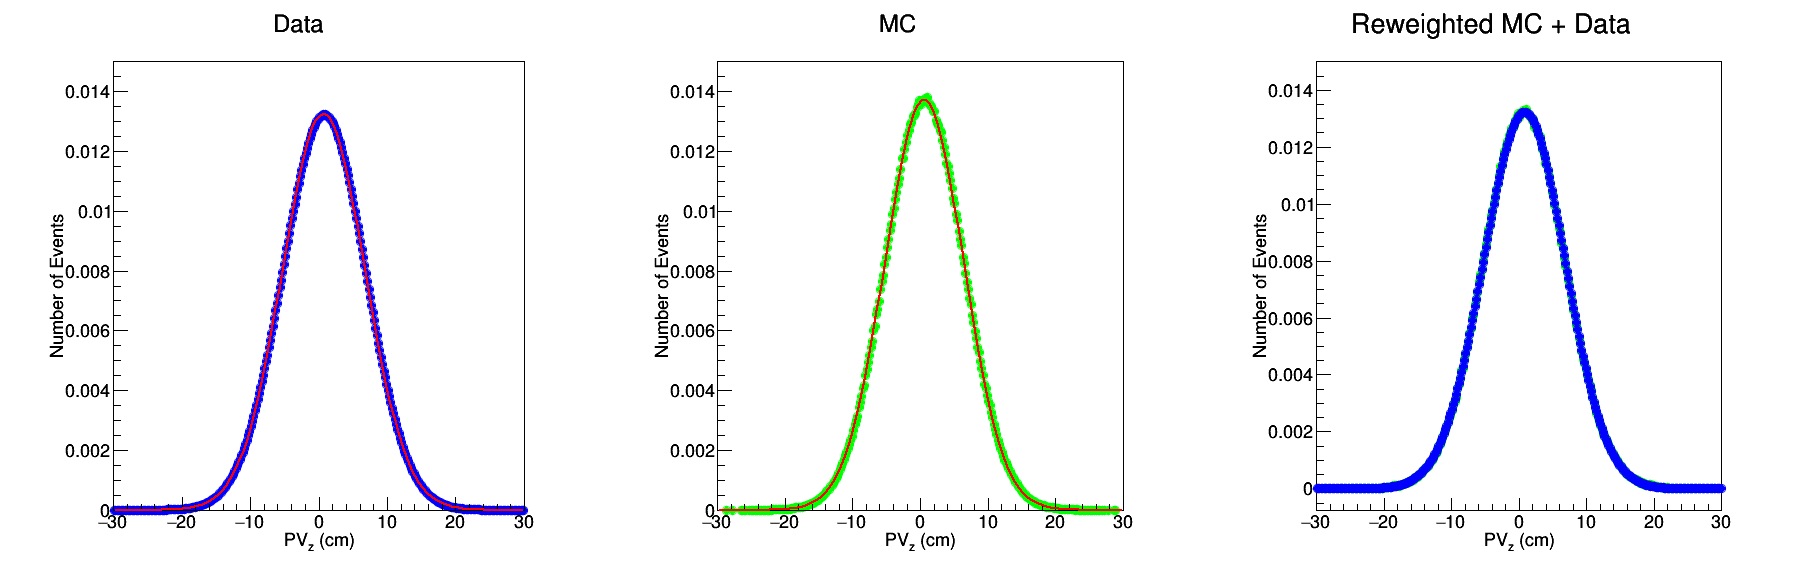
\includegraphics[width= 0.97\textwidth]{Plots/MCReweight/PVz/BPPVZMCData.png}
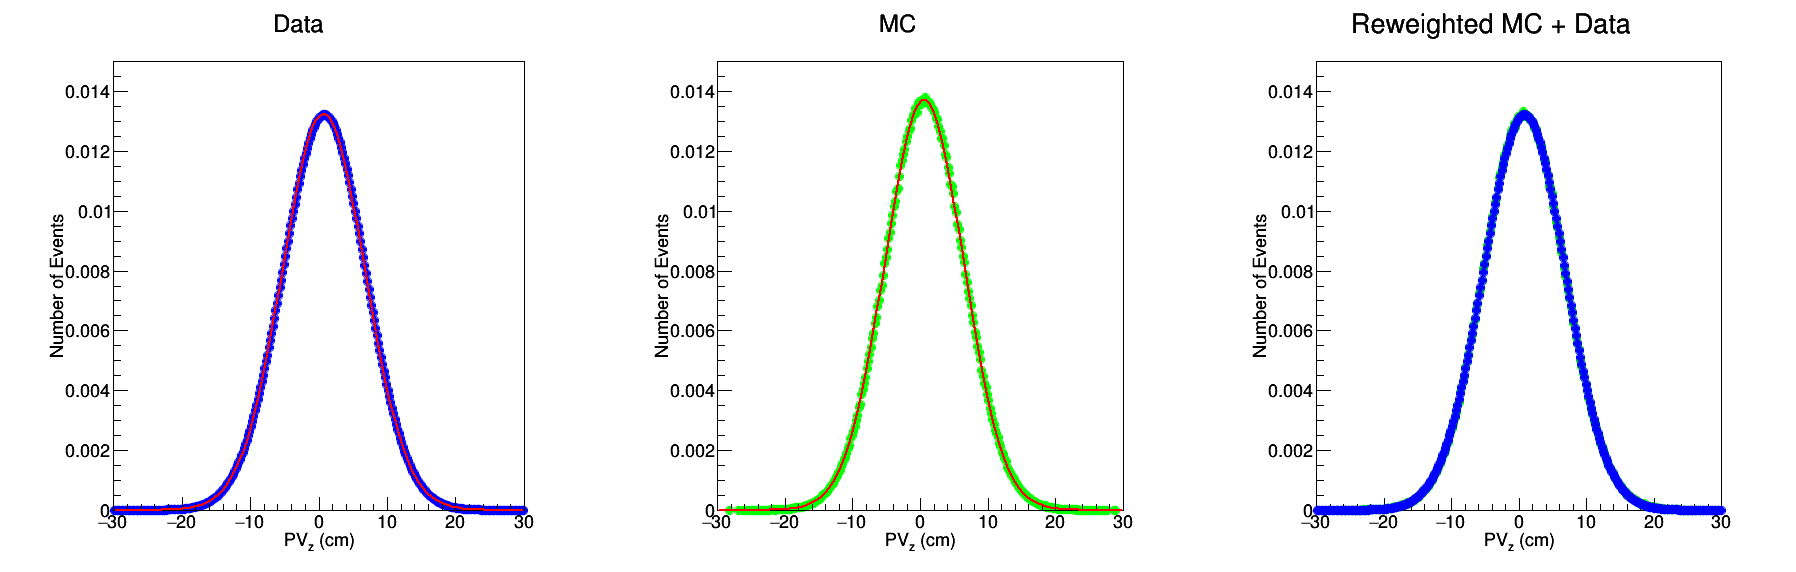
\includegraphics[width= 0.97\textwidth]{Plots/MCReweight/PVz/BsPVZMCData.png}
\caption{ 
On the left, \PBzs primary vertex z position (PVz) spectrum obtained in pp data (geen marker), fitted with a gaussian function (red line). On the middle, the same but for the MC simulations. One the right is the MC and data after reweighting the MC to data with ratio of data-to-MC Gaussian Fits. 
}
\label{fig:datamc-pvz-pp}
\end{center}
\end{figure}

\clearpage

In this case, we can see that there is no need to reweight PVz due to the excellent data MC agreement.
\clearpage

